% ============================================================================
% Appendix F — Extended Analysis
% ============================================================================

\section{Extended analysis}
\label{app:extended_analysis}

This appendix provides additional analyses that complement the main experiments. All figures are derived from existing training logs and saved trajectory data; no additional GPU experiments were run.

\subsection{State Channel dynamics}
\label{app:sc_dynamics}

Figure~\ref{fig:sc_dynamics} tracks three State Channel signals over training: SC progress (mean progress score on on-policy trajectories), SC coverage (fraction of trajectory states matched in the expert progress map), and bonus/reward ratio (SC bonus relative to environment reward). Across all four settings, SC progress and coverage increase over training as the on-policy agent visits more expert-like states. The bonus/reward ratio decreases as the environment reward grows: SC provides dense signal when it is most needed (early training) and recedes as the real reward becomes informative.

\begin{figure}[h]
\centering
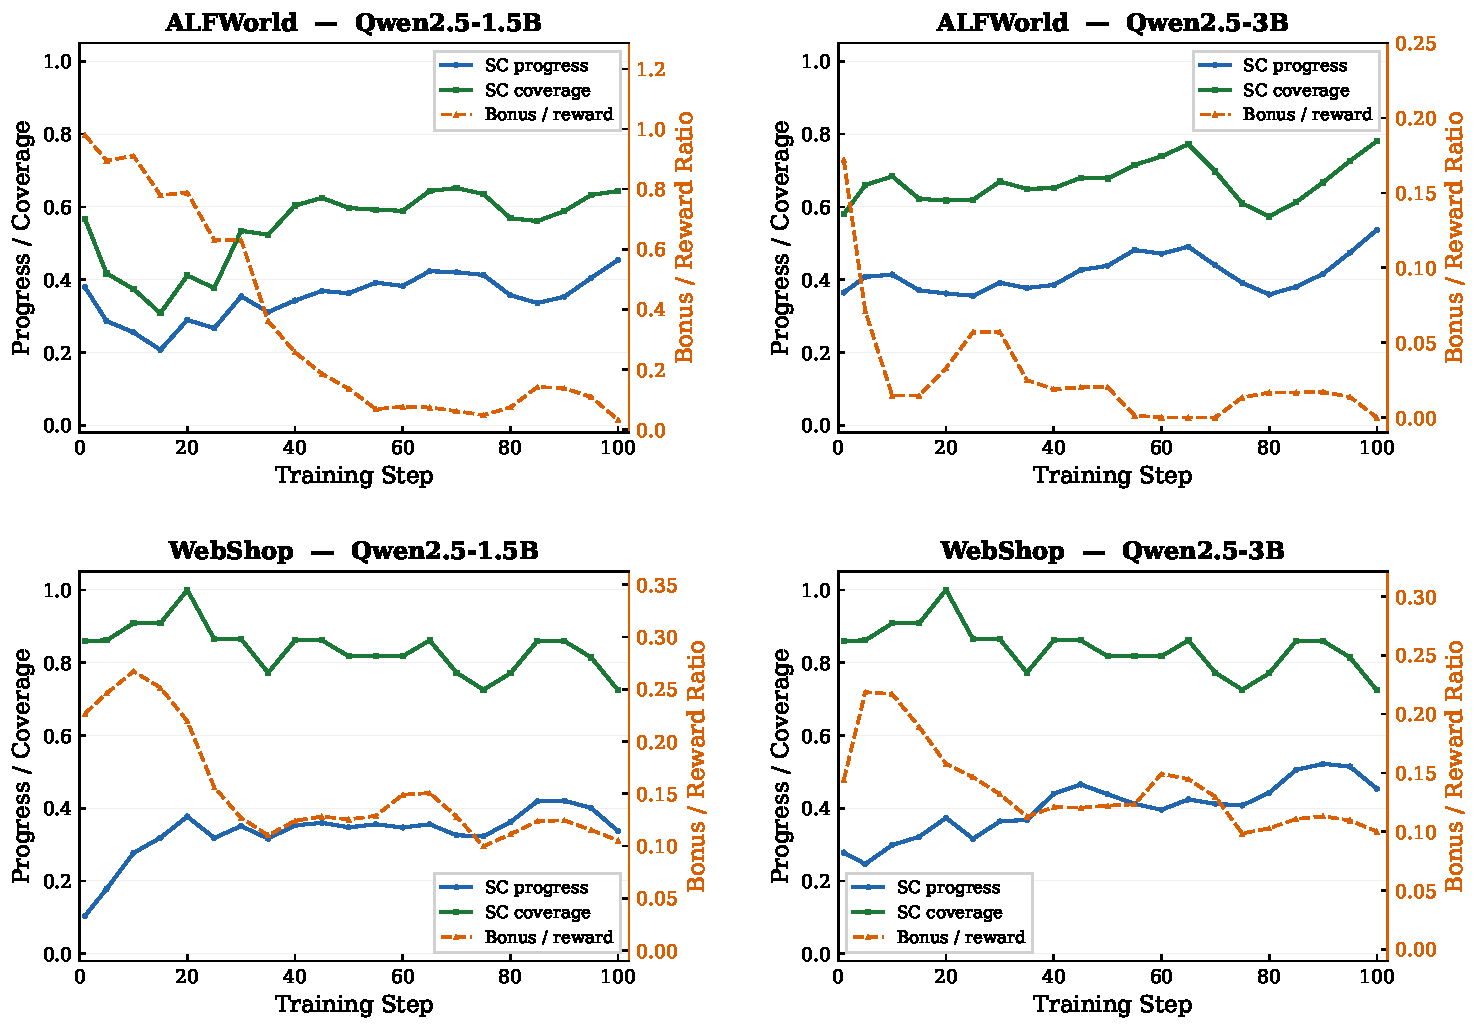
\includegraphics[width=\linewidth]{figures/fig_sc_dynamics.pdf}
\caption{\textbf{State Channel dynamics.} SC progress (blue) and coverage (green) increase as the agent improves; the bonus/reward ratio (orange, right axis) decreases as environment reward grows.}
\label{fig:sc_dynamics}
\end{figure}

\subsection{Reward decomposition}
\label{app:reward_decomp}

Figure~\ref{fig:reward_decomp} decomposes the mean total reward for on-policy DUET trajectories into three components: environment reward, SC trajectory-level bonus, and SC step-level deltas. In early training, the SC components provide the majority of the reward signal (especially visible on ALFWorld 1.5B and WebShop). As training progresses, environment reward dominates, confirming that SC reward shaping provides a useful cold-start signal without distorting the converged policy's reward landscape.

\begin{figure}[h]
\centering
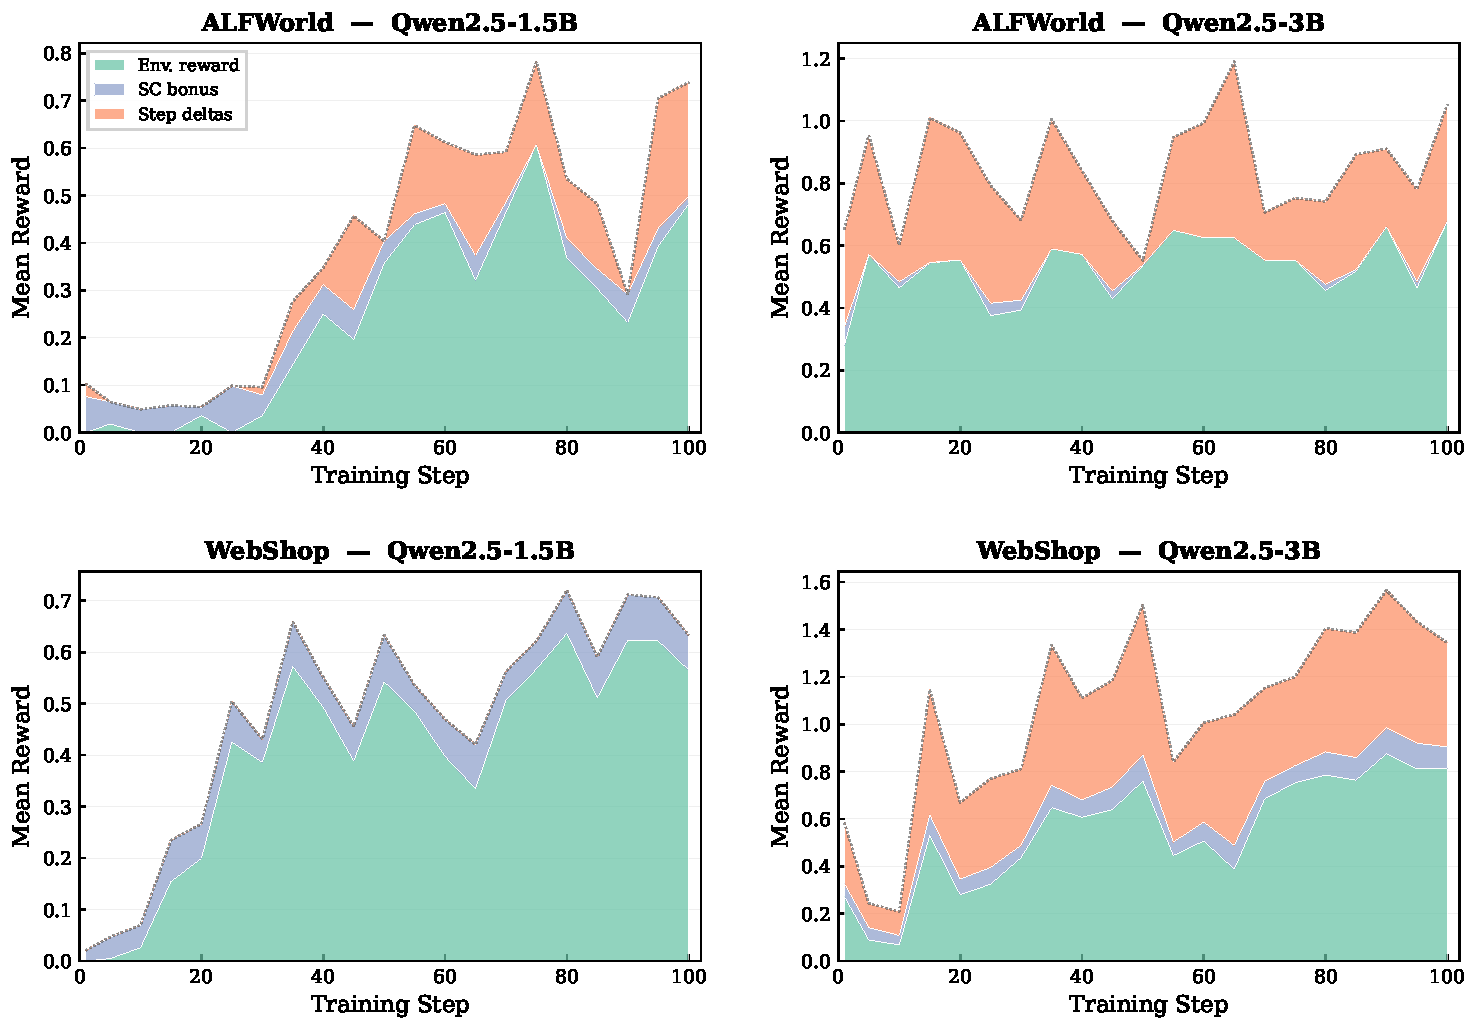
\includegraphics[width=\linewidth]{figures/fig_reward_decomposition.pdf}
\caption{\textbf{Reward decomposition} over training. Green: environment reward. Blue: SC bonus. Orange: step deltas. SC components dominate early, environment reward dominates late.}
\label{fig:reward_decomp}
\end{figure}

\subsection{Entropy comparison across methods}
\label{app:entropy}

Figure~\ref{fig:entropy} compares on-policy token entropy across all methods. DUET generally maintains higher or competitive entropy compared to baselines, suggesting that its dual-channel design preserves exploration diversity. This is most visible on ALFWorld 1.5B, where GRPO's entropy collapses to $0.02$ while DUET sustains $0.12$---DUET's dense SC reward signal provides sufficient learning gradient without requiring the policy to collapse its exploration.

\begin{figure}[h]
\centering
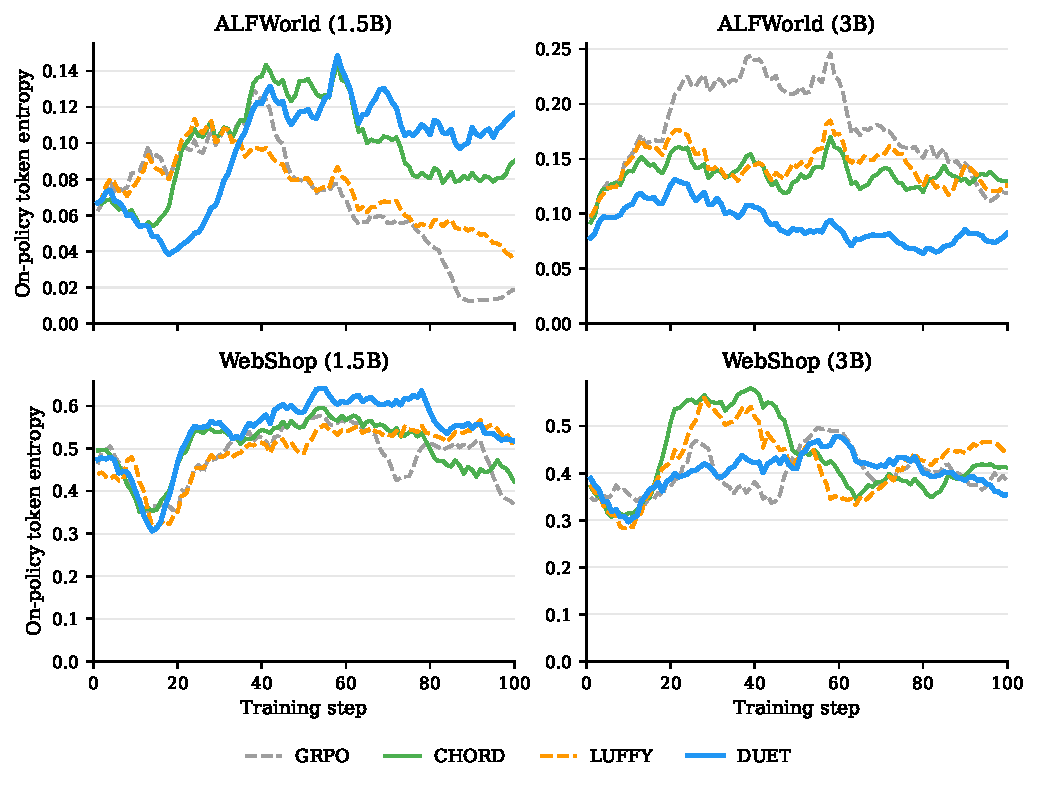
\includegraphics[width=\linewidth]{figures/fig_entropy_comparison.pdf}
\caption{\textbf{On-policy token entropy} over training. DUET maintains higher entropy than GRPO in most settings, suggesting better preservation of exploration diversity.}
\label{fig:entropy}
\end{figure}

\subsection{Per-task-type breakdown (ALFWorld)}
\label{app:task_types}

ALFWorld comprises six task types requiring different manipulation chains. Figure~\ref{fig:task_types} decomposes success rate by task type for each method. At 1.5B, DUET leads on all six types, with the largest margins on multi-step tasks (Clean: $52\%$ vs.\ $13\%$ for CHORD; Cool: $29\%$ vs.\ $17\%$). These tasks require chains of intermediate actions (e.g., find $\to$ pick up $\to$ go to sink $\to$ clean $\to$ go to destination $\to$ put), where the State Channel's step-level progress bonuses are most informative. At 3B, the gap narrows as all teacher-mixing methods benefit from stronger base capabilities, but DUET still leads overall. One notable exception is Pick Two at 3B, where GRPO outperforms all teacher-mixing methods ($51\%$ vs.\ DUET's $38\%$), suggesting that teacher demonstrations may not always be beneficial for tasks requiring broad combinatorial exploration.

\begin{figure}[h]
\centering
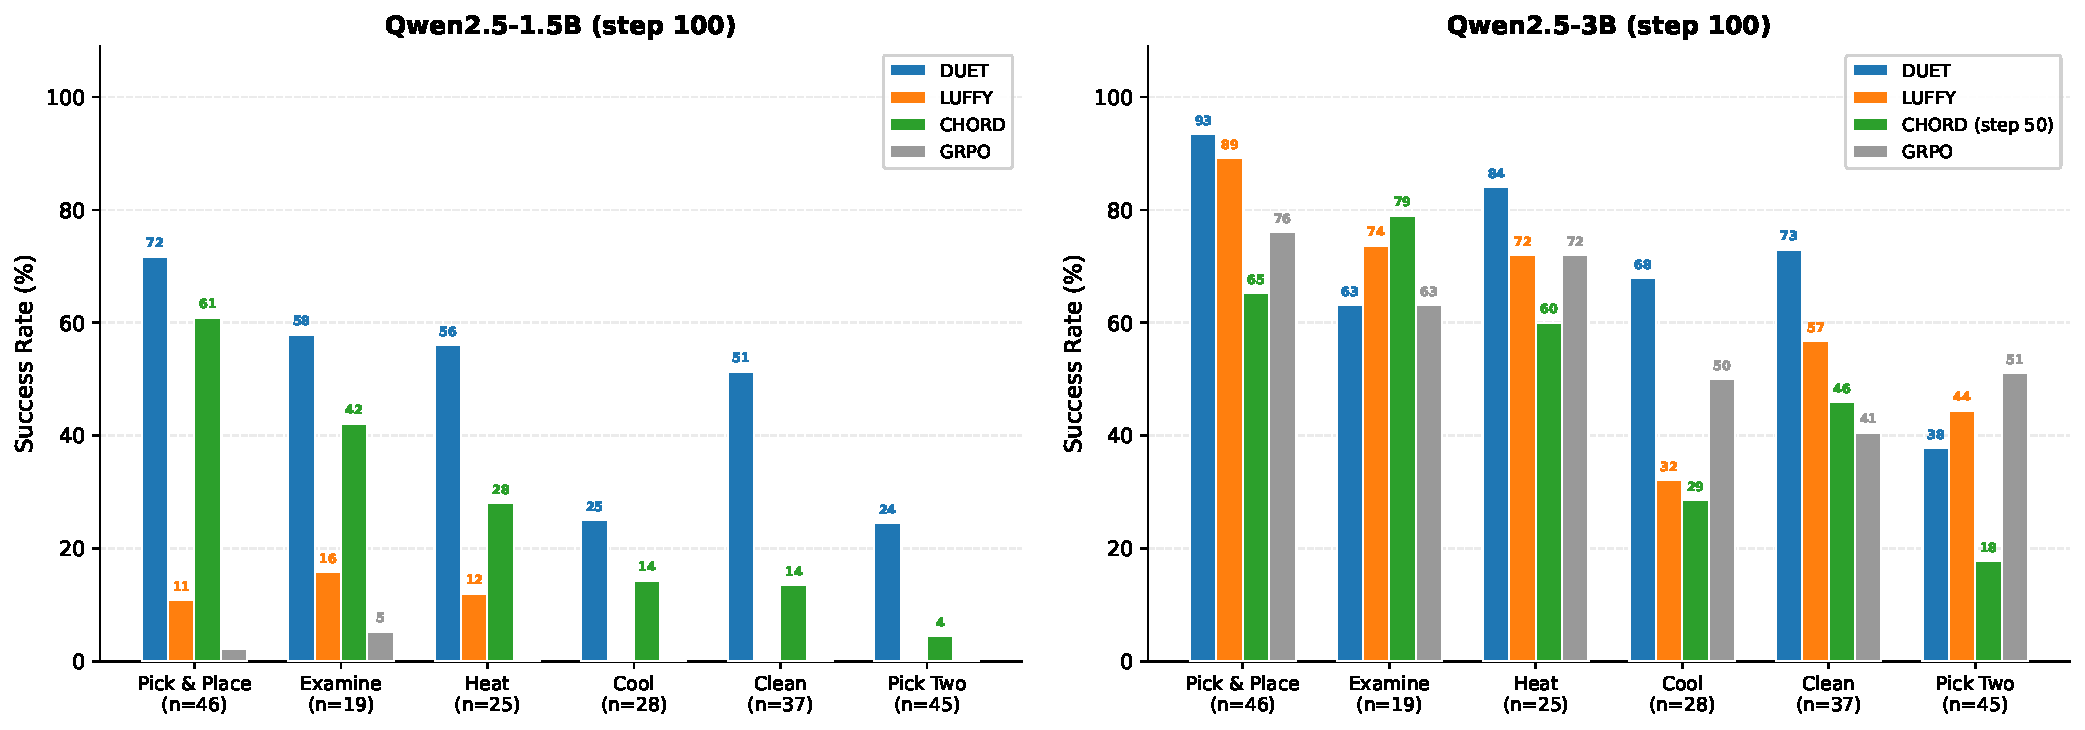
\includegraphics[width=\linewidth]{figures/fig_task_type_breakdown.pdf}
\caption{\textbf{Per-task-type success rate} on ALFWorld. DUET leads across all task types at 1.5B, with the largest gains on multi-step manipulation tasks (Cool, Clean).}
\label{fig:task_types}
\end{figure}
